\section{Dynamic Time Warping}
\label{sec:dtw}

This section covers works related to Dynamic Time Warping for time series.

\subsection{Definition}


Dynamic Time Warping (DTW,~\cite{sakoe1978dynamic}) is a similarity measure
between time series.
Consider two time series $\mathbf{x}$ and
$\mathbf{x}^\prime$ of respective lengths $n$ and
$m$.
Here, all elements $x_i$ and $x^\prime_j$ are assumed to lie in the same
$p$-dimensional space and the exact timestamps at which observations occur are
disregarded: only their ordering matters.

\subsubsection{Optimization Problem}

In the following, a path $\pi$ of length $K$ is a
sequence of $K$ index pairs
$\left((i_0, j_0), \dots , (i_{K-1}, j_{K-1})\right)$.

DTW between $\mathbf{x}$ and $\mathbf{x}^\prime$ is formulated as the following
optimization problem:

\begin{equation}
DTW(\mathbf{x}, \mathbf{x}^\prime) =
    \min_{\pi \in \mathcal{A}(\mathbf{x}, \mathbf{x}^\prime)}
        \sqrt{ \sum_{(i, j) \in \pi} d(x_i, x^\prime_j)^2 }
\label{eq:dtw}
\end{equation}

where $\mathcal{A}(\mathbf{x}, \mathbf{x}^\prime)$ is the set of all admissible
paths, \emph{i.e.} the set of paths $\pi$ such that:

\begin{itemize}
\item $\pi$ is a sequence $[\pi_0, \dots , \pi_{K-1}]$ of index pairs
  $\pi_k = (i_k, j_k)$ with $0 \leq i_k < n$ and $0 \leq j_k < m$
\item $\pi_0 = (0, 0)$ and $\pi_{K-1} = (n - 1, m - 1)$
\item for all $k > 0$ , $\pi_k = (i_k, j_k)$ is related to
  $\pi_{k-1} = (i_{k-1}, j_{k-1})$ as follows:
  \begin{itemize}
  \item $i_{k-1} \leq i_k \leq i_{k-1} + 1$
  \item $j_{k-1} \leq j_k \leq j_{k-1} + 1$
\end{itemize}
\end{itemize}

Here, a path can be seen as a temporal alignment of time series and the optimal
path (as presented in Figure~\ref{fig:dtw}) is such that
Euclidean distance between aligned (\emph{ie.} resampled) time series is
minimal.

\begin{figure}[t]
\centering
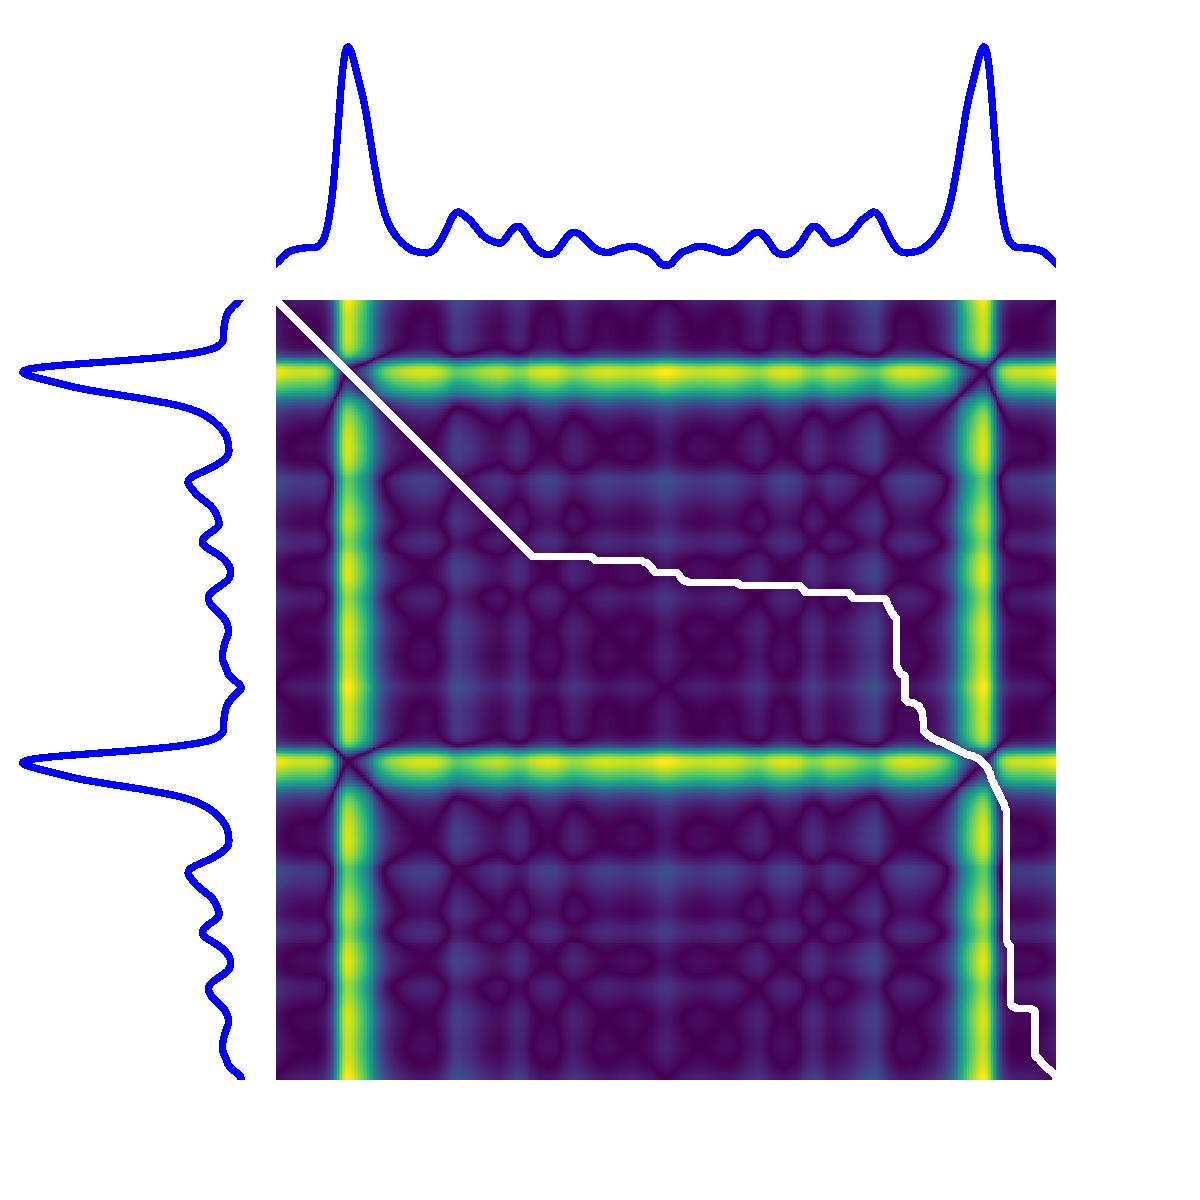
\includegraphics[width=.4\textwidth]{fig/dtw}
\caption{DTW path (in white) for a given pair of time
series, shown on top of the cross-similarity matrix that stores
$d(x_i, {x}^\prime_j)$
values. \label{fig:dtw}}
\end{figure}

\subsubsection{Algorithmic Solution}

There exists an $O(mn)$ algorithm to compute the exact optimum for this
problem, assuming computation of $d(\cdot,\cdot)$ is $O(1)$
(see Algorithm~\ref{algo:dtw}).

\begin{algorithm}[t]
 \caption{DTW algorithm. For the sake of simplicity, out-of-bounds accesses to $C$ are assumed to return $\infty$.}
 \label{algo:dtw}
 \KwData{$(\mathbf{x}, \mathbf{x}^\prime)$ : a pair of time series}
 \For{$i$ = 0..$n-1$}{
   \For{$j$ = 0..$m-1$}{
     dist = $d(x_i, x^\prime_j)^2$ \\
       \eIf{$i$ == 0 \textup{\textbf{and}} $j$ == 0}{
         $C_{i, j} = dist$
       }{
         $C_{i, j} = dist + \min(C_{i-1, j}, C_{i, j-1}, C_{i-1, j-1})$
       }
    }
  }
  \Return $\sqrt{C_{n - 1, m - 1}}$
\end{algorithm}


\subsubsection{Properties}

Dynamic Time Warping holds the following properties:

\begin{itemize}
\item $\forall \mathbf{x}, \mathbf{x}^\prime, DTW(\mathbf{x}, \mathbf{x}^\prime) \geq 0$
\item $\forall \mathbf{x}, DTW(\mathbf{x}, \mathbf{x}) = 0$
\end{itemize}

However, mathematically speaking, DTW is not a valid metric since it
satisfies neither the triangular inequality nor the identity of indiscernibles.

\subsubsection{Setting additional constraints}

The set of temporal deformations to which DTW is invariant can be reduced by
imposing additional constraints on the set of acceptable paths.
Such constraints typically consist in forcing paths to stay close to the
diagonal.

The Sakoe-Chiba band is parametrized by a radius $r$ (number of
off-diagonal elements to consider, also called warping window size sometimes),
as illustrated in Figure~\ref{fig:sakoe}.
The Itakura parallelogram sets a maximum slope $s$ for alignment
paths, which leads to a parallelogram-shaped constraint (see Figure~\ref{fig:itakura}).

\begin{figure}[t]
    ~~~~~~~~~
    \begin{subfigure}[b]{0.35\textwidth}
         \centering
         
\includegraphics[width=\textwidth]{fig/sakoe}
         \caption{Sakoe-Chiba band of radius $r=3$}
         \label{fig:sakoe}
     \end{subfigure}
     \hfill
     \begin{subfigure}[b]{0.35\textwidth}
          \centering
          
\includegraphics[width=\textwidth]{fig/itakura}
          \caption{Itakura parallelogram of slope $s=2$}
          \label{fig:itakura}
      \end{subfigure}
      ~~~~~~~~~
    \caption{Global constraints for Dynamic Time Warping.}
\end{figure}

\subsection{Constrained Dynamic Time Warping}

In this section, we present a method to regularize Dynamic Time Warping
by setting constraints on the length of the admissible warping
paths~\cite{zhang2017dynamic}.%
\footnote{This work is a part of Zheng Zhang's PhD thesis. It was performed
during Zheng's stay at LETG in 2015-2016.
I was not directly involved in the supervision Zheng's PhD thesis.}

\subsubsection{Formulation and Optimization}

As discussed above, a common way
to restrict the set of admissible temporal distortions for Dynamic Time Warping
consists in forcing paths to stay close to the diagonal through the use of
Sakoe-Chiba band or Itakura parallelogram constraints.
A limitation of these global constraints is that they completely
discard some regions of the alignment matrix \emph{a priori}
(\emph{i.e.} regardless of the involved data).

To alleviate this limitation, we propose Limited warping path length DTW (LDTW)
that adds a path length constraint to the DTW
optimization problem such that a path is said admissible for our method iff:

\begin{itemize}
\item it is an admissible DTW path;
\item its length $K$ is lower or equal to a user-defined bound $K_\text{max}$.
\end{itemize}

We have proposed an algorithm that stores, at each step $(i, j)$, optimal
alignment scores for all admissible alignment path lengths.
This gives the general LDTW algorithm presented in Algorithm~\ref{algo:ldtw}.

\begin{algorithm}[t]
 \caption{LDTW algorithm. For the sake of simplicity, out-of-bounds accesses to $C$ are assumed to return $\infty$.}
 \label{algo:ldtw}
 \KwData{$(\mathbf{x}, \mathbf{x}^\prime)$ : a pair of time series, $K_\text{max}$: an upper bound on the path length}
 \For{$i$ = 0..$n-1$}{
   \For{$j$ = 0..$m-1$}{
     \texttt{// Set infinite cost for non-admissible lengths:} \\
     $C_{i, j, :} = (\infty, \cdots , \infty)$ \\
     dist = $d(x_i, x^\prime_j)^2$ \\
     \texttt{// The core difference with DTW is the following loop:} \\
     \For{$l \in \mathrm{admissible\_lengths}(i, j, K_\text{max})$}{
       \eIf{$i$ == 0 \textup{\textbf{and}} $j$ == 0}{
         $C_{i, j, l} = dist$
       }{
         $C_{i, j, l} = dist + \min(C_{i-1, j, l-1}, C_{i, j-1, l-1}, C_{i-1, j-1, l-1})$
       }
 	  }
    }
  }
  \Return $\sqrt{\min_{k} C_{n - 1, m - 1, k}}$
\end{algorithm}


The question is then to compute the set
\texttt{admissible\_lengths}$(i, j, K_\text{max})$.
We have shown that this set can be computed explicitly and that its cardinal
is $O(\min(i, j))$.
Overall, we have a $O(mn^2 + nm^2)$ complexity for this exact algorithm.

\subsubsection{Empirical Observations}

First, one can see in Figure~\ref{fig:ldtw} that the resulting alignments
effectively limits the number of singularities in the obtained alignments as
compared to DTW.

\begin{figure}[t]
    \begin{subfigure}[b]{\textwidth}
         \centering
         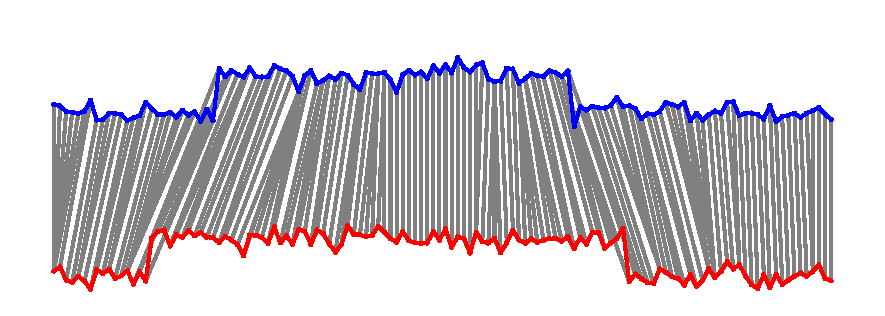
\includegraphics[width=.8\textwidth]{fig/dtw_warping_length}
         \caption{LDTW matches}
     \end{subfigure}
     \begin{subfigure}[b]{\textwidth}
          \centering
          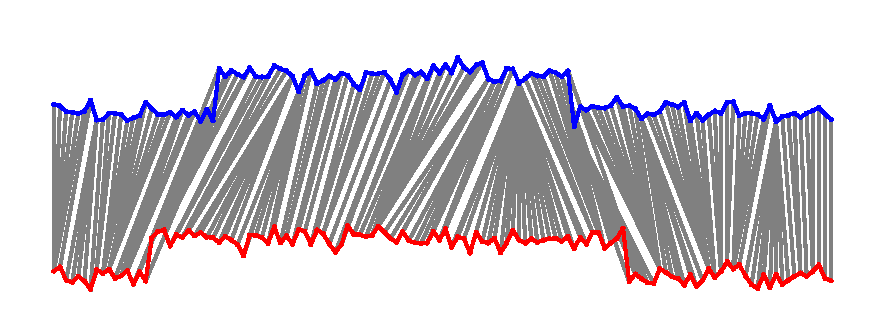
\includegraphics[width=.8\textwidth]{fig/dtw_warping_length_b}
          \caption{DTW matches}
      \end{subfigure}
    \caption{Compared matches obtained with DTW and its
    warping-length-constrained variant LDTW. Note the comparatively smaller
    temporal distortions induced by LDTW.}
    \label{fig:ldtw}
\end{figure}

Moreover, our experiments on UCR Time Series Datasets~\cite{ucr} show that
this similarity measure, when used in a 1-Nearest Neighbor Classifier, leads to
a higher accuracy than other constrained DTW variants
(Sakoe-Chiba band and Itakura parallelogram).

\subsection{DTW Alignment as an Adaptive Resampling Strategy}

In this section, we present a method that uses Dynamic Time Warping (DTW)
on multimodal time series, \emph{i.e.} time series that are made of several
features recorded over time.
The method relies on the assumption that one of the considered modalities
(called
reference modality in the following) can be used as a reference to (temporally)
realign other modalities~\cite{dupas:halshs-01228397}.
It has been used in the context of hydrological measurements to align pollutant
concentration profiles based on discharge time series.%
\footnote{This work is a part of Rémi Dupas' PhD thesis (in Environment
Sciences).
I was not directly involved in the supervision of Rémi's PhD thesis.}

This approach can be seen as the DTW counterpart of other works that rely on
Optimal Transport for Domain Adaptation~\cite{courty:hal-02112785}.
One significant difference, however, is that it relies on a reference modality
for
alignment.
This design choice is guided by our application context.

\subsubsection{Motivating Use Case}

Phosphorus (P) transfer during storm events represents a significant part of
annual P loads in streams and contributes to eutrophication in downstream water
bodies. To improve understanding of P storm dynamics, automated or
semi-automated methods are needed to extract meaningful information from
ever-growing water quality measurement datasets.

Clustering techniques have proven useful for identifying seasonal storm
patterns and thus for increasing knowledge about seasonal variability in storm
export mechanisms (\emph{e.g.},~\cite{aubert:halshs-00906292}).
Clustering techniques usually require calculating distances between pairs of
comparable points in multiple time series. For this reason, direct clustering
(without using hysteresis-descriptor variables) of high-frequency storm
concentration time series is usually irrelevant because the lengths of recorded
time series (number of
measurement points) might differ and/or measurement points may have different
positions relative to the hydrograph (flow rise and recession); hence, it is
difficult to calculate a distance between pairs of comparable points.

The aim of this study was to develop a clustering method that overcomes this
limit and test its ability to compare seasonal variability of P storm dynamics
in two headwater watersheds. Both watersheds are ca. 5 km$^2$, have similar
climate and geology, but differ in land use and P pressure intensity.

\subsubsection{Alignment-based Resampling Method}

In the above-described setting, we have access to one modality (discharge,
commonly denoted $Q$) that is representative of the evolution of the flood.
Temporal realignment based on this modality allows to overcome three
difficulties that can arise when comparing storm-event data.
Indeed, time series can have

\begin{enumerate}
\item different starting times due to the discharge threshold at which the
samplers were triggered,
\item different lengths, and
\item differences in phase that yield different temporal localizations of the
discharge peak.
\end{enumerate}

To align time series, we use the path associated with DTW.
This matching path can be viewed as the optimal way to perform point-wise
alignment of time series.

For each discharge time series $\mathbf{x}^{(i)}_\text{Q}$, we compute the
matching path $\pi_\text{Q}$ and use it to find the optimal alignment wrt.
the same reference discharge time series $\mathbf{x}^\text{ref}_\text{Q}$.
The reference discharge time series used in this study is chosen
as a storm event with full coverage of flow rise and flow recession phases.
Alternatively, one could choose a synthetic idealized storm hydrograph.

We then use barycentric mapping based on the obtained matches to realign other
modalities to the timestamps of the reference time series, as shown in
Figure~\ref{fig:dtw_da}.

\begin{figure}[t]
    \begin{subfigure}[b]{\textwidth}
         \centering
         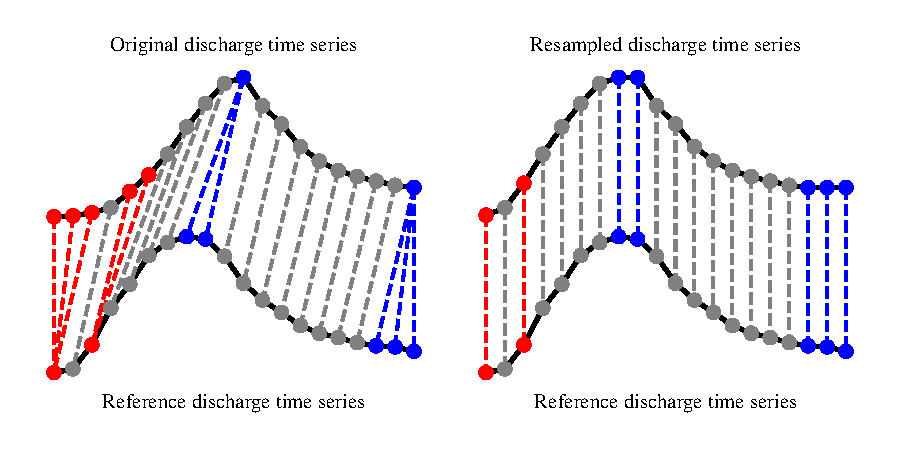
\includegraphics[width=.7\textwidth]{fig/dtw_da}
     \end{subfigure}
      \begin{subfigure}[b]{\textwidth}
           \centering
           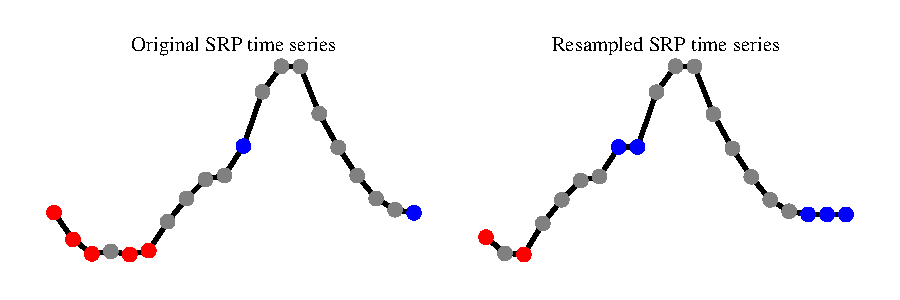
\includegraphics[width=.7\textwidth]{fig/dtw_da_b}
       \end{subfigure}
    \caption{Adaptive resampling strategy. Top row: A discharge time series is
    resampled so that its timestamps match those of a reference one. Bottom row:
    The same temporal transformation is applied to all other modalities
    (\emph{e.g.} SRP concentration) of the given sample.}
    \label{fig:dtw_da}
\end{figure}

At this point, each time series is transformed to series of $n$
$p$-dimensional measurements, where $n$ is the length of the
reference discharge time series and $p$ is the number of water quality
parameters considered in the study (\emph{i.e.} all modalities except the
discharge).
In a second step, a standard $k$-means algorithm is used to cluster
realigned time series.
Note that a Euclidean distance can be used for clustering since time series
have already been temporally realigned; hence, time-sensitive metrics (such as
DTW) are no longer needed.

This method proved useful to extract meaningful clusters and an \emph{a posteriori}
analysis of the clusters enabled to identify the export dynamics of pollutants
in different geographical areas of the study sites, which then led to management
recommendations, as detailed in~\cite{dupas:halshs-01228397}.

\subsection{DTW with Global Invariances}
\label{sec:dtw_gi}

In this work we address the problem of comparing time series while taking
into account both feature space transformation and temporal variability.
The proposed framework combines a latent global transformation of the feature
space with the widely used Dynamic Time Warping (DTW).
This work is available as preprint~\cite{vayer2020time}.%
\footnote{This work is part of Titouan Vayer's PhD thesis.
We are co-supervising Titouan together with Laetitia Chapel and Nicolas Courty.}

\subsubsection{Definition}

Let $\mathbf{x}$ and $\mathbf{x^\prime}$ be two time series of respective
lengths $n$ and $m$.
Here, features from both time series are not assumed to lie in the same ambient
space, but it is assumed that features from $\mathbf{x}$ lie in $\mathbb{R}^p$
while features from $\mathbf{x^\prime}$ lie in $\mathbb{R}^{p'}$
In the following, we assume $p \geq p'$ without loss of generality.
In order to allow comparison between time series $\mathbf{x}$ and
$\mathbf{x^\prime}$,
we will optimize on a family of functions $\mathcal{F}$ that map features from
$\mathbf{x^\prime}$ onto the feature space in which features from $\mathbf{x}$
lie. More formally, we define Dynamic Time Warping with Global Invariances
(DTW-GI) as the solution of the following joint optimization problem:

\begin{equation}
    \text{DTW-GI}(\mathbf{x}, \mathbf{x^\prime}) =
        \min_{f \in \mathcal{F}, \pi \in \mathcal{A}(\mathbf{x}, \mathbf{x^\prime})}
            \sqrt{ \sum_{(i, j) \in \pi} d(x_i, f(x^\prime_j))^2 } \, ,
    \label{eq:dtwgi}
\end{equation}

where $\mathcal{F}$ is a family of functions from $\mathbb{R}^{p^\prime}$ to
$\mathbb{R}^{p}$.

This similarity measure estimates both temporal alignment and feature space
transformation between time series simultaneously, allowing the alignment of
time series when the similarity should be defined up to a global transformation.
Time series do not have to lie in the same ambient space, as presented in
Figure~\ref{fig:dtw-gi}.

\begin{figure}[t]
    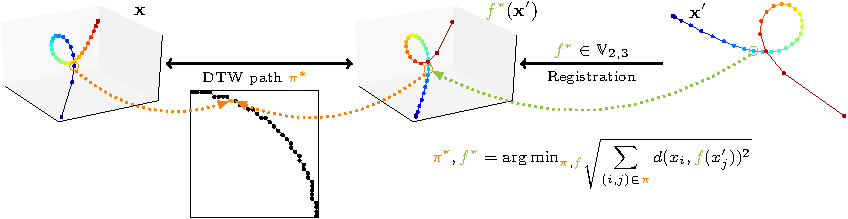
\includegraphics[width=\linewidth]{fig/dtw_gi_cropped}
    \caption{DTW-GI aligns time series by optimizing on temporal alignment
    (through Dynamic Time Warping) and feature space transformation (denoted
    $f$ here). Time series represented here are color-coded trajectories, whose
    starting (resp. end) point is depicted in blue (resp. red).}
    \label{fig:dtw-gi}
\end{figure}



\subsubsection{Optimization}

Optimization of the quantity in Equation \eqref{eq:dtwgi} can be performed
\emph{via} Block Coordinate Descent.
In a nutshell, optimization alternates between the following two steps:

1. for a fixed $f$, determine the optimal alignment path $\pi$ using the DTW
algorithm;
2. for a fixed path $\pi$, the optimal map $f$ (when $\mathcal{F}$ is the
Stiefel manifold) is obtained through Singular Value Decomposition.

Interestingly, this optimization strategy where we alternate between time
series alignment, \emph{i.e.} time correspondences between both time series, and
feature space transform optimization can be seen as a variant of the Iterative
Closest Point (ICP) method in image registration~\cite{CHEN1992145}, in
which  nearest neighbors are replaced by matches resulting from DTW alignment.

We also introduce soft counterparts following the definition of softDTW
from~\cite{cuturi2017soft}.
In this case, optimization consists in gradient descent and a wider variety of
feature space transformation families can be considered.

\begin{figure}[t]
	\centering
	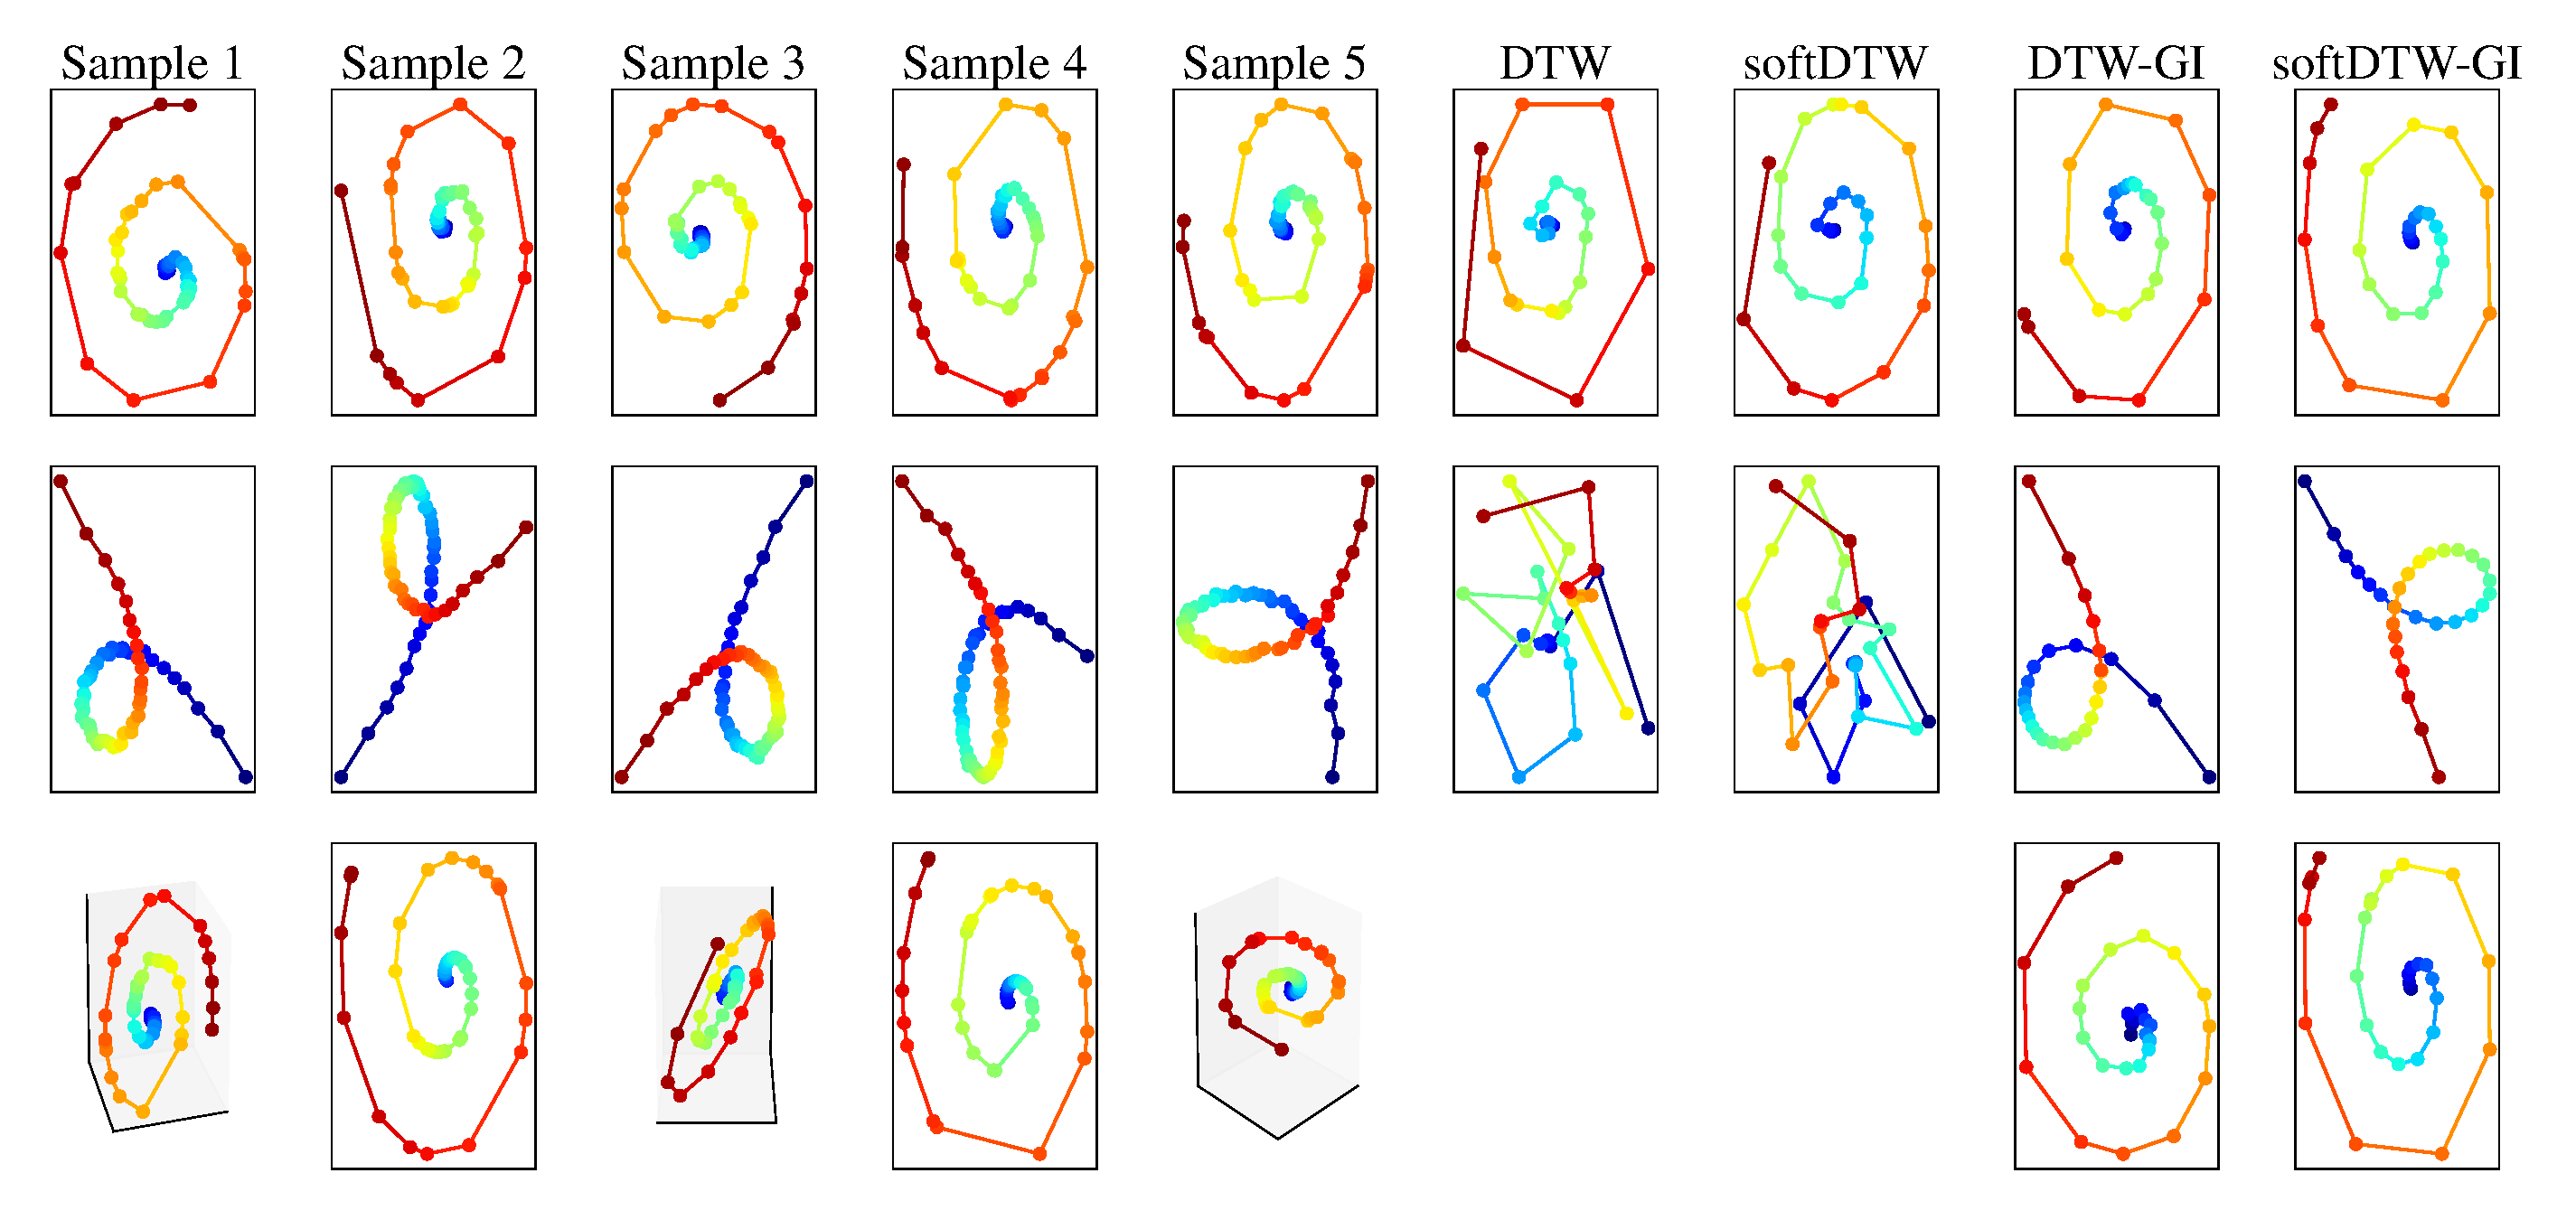
\includegraphics[width=\linewidth]{fig/barycenter_toys_allinone}
	\caption{
		Barycenter computation using (i) DTW and softDTW baseline approaches, (ii) their rotation-invariant counterparts DTW-GI and soft-DTW-GI.
		Each row correspond to a different dataset, and the latter one contains both 2d and 3d trajectories, hence cannot be tackled by any baseline method.
		Trajectories are color-coded from blue (beginning of the series) to red (end of the series).
		\label{fig:dtw_gi_bary}
	}
\end{figure}

Figure~\ref{fig:dtw_gi_bary} presents examples of barycenters obtained with
various DTW-based barycenter computation methods to illustrate the interest of
our approach.
We validate the utility of these similarity measures on real world
datasets on the tasks of human motion prediction (where motion is captured under
different points of view) and cover song identification (where song similarity
is defined up to a key transposition).
In both these settings, we observe that joint optimization on feature space
transformation and temporal alignment improves over standard approaches that
consider these as two independent steps.

